\usepackage{float}
\chapter{METHODOLOGY}
{\baselineskip=2\baselineskip

This chapter describes the methodological framework used in developing the
machine learning--based watermelon ripeness detection system. It details the research
design adopted in the study, the requirements analysis, and the procedures for data
gathering and acquisition. The chapter further explains the image collection process, data
preprocessing techniques, model training and validation, and system evaluation methods.
These procedures were systematically implemented to ensure accurate ripeness
classification, model reliability, and consistency of results under real-world agricultural
conditions.

\section{Research Design \& Procedure}

The proposed research will utilize the Modified Waterfall Methodology, which
has a linear and sequential structure, but with overlapping phases or ``feedback loops''.
This methodology is best for software-hardware systems, which is fit for our proposed
study.

The research design chosen for this study was the System Development Life
Cycle (SDLC), specifically the modified Waterfall Model in Figure~2. The sequential
structure of the Waterfall Model---which consists of requirements gathering,
requirements analysis, system design \& development, and testing---aligns with the
implementation of object detection and audio classification for pre-harvest watermelons.
Additionally, with the modified Waterfall Model, an option to go back to the previous
phase is available in the event that errors occur in the current phase.

Because the core requirements of the system such as the established resonant
frequency (Wongkalasin et al., 2023) and the efficacy of SVM and ensemble modeling
(Arboleda et al., 2020; Qi et al., 2024) are already well defined, a structure and
sequential framework provides the necessary discipline for the development. However,
the ``modified'' aspect of this model is critical for addressing the transition from the
``controlled lab conditions'' to the ``real-world field conditions'' targeted in our study
since we are dealing with pre-harvest watermelons, meaning they are still grown. By
incorporating feedback loops between phases, this SDLC allows for essential
backtracking, which is particularly vital when integrating acoustic sensors and image
analysis, as both may require iterative recalibration during development and integration
phase. Furthermore, the model respects the inherent physical dependency of the system
itself, where the collection of dataset is logically gated by the successful design and
integration of the microphone, camera and microcontroller since we will be needing it to
collect audio and image data. This ensures that each stage, from hardware-software to
integration phase, undergoes rigorous verification before progressing, mitigating the risk
of cascading errors in the final system. By structuring the development this way, the
Waterfall Model directly supports the methodological rigor, flexibility, and practical
reliability required to deliver a system capable of addressing the persistent issue of
manual pre-harvest watermelon inspection in agricultural farms.

\begin{figure}[ht]
	\centering
	
\includegraphics[width=0.65\linewidth]{Thesis Format (LaTEX)/figures/modified-waterfall-model.png}
	\caption{The Modified Waterfall Model}
	\label{fig:waterfall}
\end{figure}

\section{Data Gathering}

The data gathering for this study will be conducted in a selected farm near
Cagayan de Oro City. The data to be collected will be through an interview with the
farmer, and sound and image samples from the watermelons planted in the farm. The
interview will help gather insights on current practices for determining watermelon
ripeness, common issues, and accuracy concerns therein. Meanwhile, sound samples will
be collected through tapping the watermelons and recording the sound using a prototype
of the proposed device. Pictures of the watermelons' tendrils will also be taken.

\section{Requirements Analysis}

Defines the essential hardware and software specifications required to develop the
watermelon ripeness detection device. By establishing the system's architecture and
functional framework, these requirements provide the technical blueprint necessary to
guide the project from conceptual design to successful implementation.

\subsection{Hardware Requirements}

\begin{itemize}

	\item \textbf{Microprocessor.} The ESP32-S3 N16R8 was selected as the primary
	microcontroller for this system. The ESP32-S3 represents a strategic pivot in
	Espressif's architecture from connectivity-first to intelligent-compute-first design,
	built on a dual-core Xtensa LX7 processor running at 240~MHz, delivering more than
	five times the computational throughput of earlier single-core ESP variants (Yan, 2025).
	The N16R8 configuration specifically provides 16~MB of external Flash and 8~MB of
	PSRAM, which directly addresses the memory demands of running concurrent audio
	buffering, FFT-based signal processing, machine learning inference, and camera frame
	capture on a single embedded unit.

	A critical hardware advantage of the ESP32-S3 over the standard
	ESP32-WROOM-32 is its dedicated LCD\_CAM peripheral, which operates independently
	of the I2S audio bus. This architectural separation allows the system to sample
	microphone input via I2S and capture camera frames simultaneously on a single board,
	eliminating the need for a secondary microcontroller solely to handle camera operations.
	Furthermore, the ESP32-S3 integrates the ESP-DSP vector instruction set and supports
	the TensorFlow Lite Micro framework, enabling on-device deployment of lightweight
	classifiers, consistent with the study's approach of exporting trained SVM or decision
	tree models as compact, hardcoded inference routines deployable without a dedicated GPU
	or cloud dependency (Yan, 2025). The chip also features native USB Serial/JTAG
	support, allowing direct firmware flashing and debugging via USB-C throughout
	development. The chosen board variant is the AI-Thinker ESP32-S3-CAM or Freenove
	ESP32-S3-WROOM, both of which pre-mount the N16R8 module with an integrated
	camera connector, minimizing soldering requirement.

	\item \textbf{Pulse Thumper.} The pulse thumper serves as the mechanical actuator
	responsible for delivering a standardized, repeatable impact to the watermelon surface,
	replacing the variability inherent in manual hand-tapping. A push-pull solenoid will be
	used for this purpose, driven by a MOSFET transistor controlled via a GPIO pin on the
	ESP32-S3. The solenoid operating voltage will be determined during the hardware
	prototyping phase through empirical testing, as the optimal voltage depends on the
	trade-off between strike force sufficient to produce a detectable acoustic response and
	the risk of surface bruising, a concern directly relevant to the non-destructive nature of
	the assessment. A 1N4007 flyback diode will be placed across the solenoid terminals to
	suppress back-EMF and protect the microcontroller from voltage spikes during switching.
	The striker tip will be fitted with a rubber damping head to replicate the damped impact
	profile of a human thumb and prevent metallic ringing artifacts from contaminating the
	recorded acoustic signal. This mechanical standardization is essential for ensuring that
	the acoustic features extracted across different measurement sessions remain comparable,
	directly addressing the subjectivity limitation of the traditional thumping technique
	identified in the problem statement.

	\item \textbf{Microphone.} The INMP441 MEMS digital microphone module was
	selected for acoustic signal capture. This component communicates over the I2S
	protocol, which maps directly to the ESP32-S3's I2S peripheral through well-documented
	Arduino and ESP-IDF libraries, eliminating the analog noise and resolution limitations
	associated with the ESP32's onboard ADC, a consideration particularly relevant given
	that the system targets resonant frequency features in the range of approximately
	100--300~Hz, where signal fidelity is critical for accurate classification (Li et al., 2025;
	Pamungkas \& Bintoro, 2021). The INMP441 provides an omnidirectional response with
	a flat frequency range from 60~Hz to 15~kHz, fully encompassing the target acoustic
	spectrum. The module will be mounted within the enclosure at a distance of approximately
	2--5~cm from the watermelon contact surface, oriented perpendicular to the strike point,
	and housed within a small acoustic chamber integrated into the enclosure design to
	attenuate ambient noise pickup during field operation.

	\item \textbf{Camera.} A compact camera module will be required to capture an image
	of the watermelon's ground spot for color-based maturity analysis. The camera will only
	need to capture a still image with sufficient color accuracy under natural outdoor lighting.
	It will be mounted on the enclosure facing downward or forward toward the fruit surface,
	as shown in the 3D model. A camera compatible for the ESP32-S3's camera connections
	will be chosen, such as the OV2624 with an extended Flexible Flat Cable (FFC).

	\item \textbf{LCD Display.} An LCD display will be used to present the ripeness
	classification result to the user. Based on the 3D model, a character or small graphical
	LCD module will be mounted on the back face of the device for easy reading during
	operation. The display will need to interface with the microprocessor over I2C or SPI
	and should be readable under outdoor lighting conditions.

	\item \textbf{Battery.} The device will be powered by a rechargeable battery housed
	within the enclosure. The voltage of the battery will be determined depending on what
	voltage the push-pull solenoid is rated, to ensure it will function sufficiently. To power
	the ESP32-S3, a Buck Converter will be used to step down the battery's voltage to the
	microcontroller's operating voltage to ensure it won't be damaged. A capacitor will be
	added to prevent a ``brownout'' on the microcontroller, where it will not get enough
	power due to the solenoid hogging the voltage. The battery will need to provide enough
	capacity for a reasonable field working session without requiring frequent recharging.

	\item \textbf{Enclosure.} Based on the 3D model, the system will be housed in a
	custom-designed handheld enclosure that integrates all components in a fixed
	layout---with the pulse thumper at the front, the microphone and camera facing the fruit,
	the microprocessor mounted internally, and the LCD display and battery at the rear. The
	enclosure will likely be 3D-printed to match the designed form factor and will need to be
	sturdy enough for regular outdoor farm use.

\end{itemize}

\subsection{Software Requirements}

\begin{itemize}

	\item \textbf{Programming Language and IDE.} The firmware and processing logic
	will be written in C/C++ using the Arduino IDE or PlatformIO, both of which have
	strong community support for ESP32 and similar boards. MicroPython will be another
	option that allows Python-style scripting directly on the microcontroller, which may
	simplify the implementation of the signal processing and classification routines. The
	development team will choose based on familiarity and which option best supports the
	audio and camera libraries available for the target board.

	\item \textbf{Signal Processing.} The signal processing pipeline will need to extract
	basic frequency-domain features from the recorded tap sound. This will involve
	computing a Fast Fourier Transform on the audio sample and identifying dominant
	frequency components that correlate with ripeness. On a microcontroller, this will be
	done using lightweight FFT libraries available for Arduino or MicroPython
	environments. The processing will not need to be complex---a small set of frequency and
	amplitude features will be sufficient as input to the classifier.

	\item \textbf{Computer Vision.} The image processing component will leverage a
	lightweight convolutional neural network (CNN) to analyze the tendril region of
	captured images and assess the wilting state, which correlates with the ripeness stage of
	the fruit. The method is designed to operate on low-resource hardware, making it
	feasible for deployment on devices without dedicated GPUs.

	\item \textbf{Machine Learning Classifier.} The classifier that combines acoustic and
	visual features to determine ripeness will be kept simple. Given the structured,
	low-dimensional nature of the feature input, a lightweight classical approach will be
	well-suited for this task. The model will be trained on a desktop computer then
	converted into a compact, hardcoded form for deployment on the microcontroller. No
	deep learning framework or complex model architecture will be required---the feature set
	will be small enough that a straightforward classifier will be adequate.

	\item \textbf{Version Control.} Git will be used to manage the project's source code
	and keep track of changes throughout development. A shared repository on a platform
	such as GitHub will allow the team to collaborate and maintain a history of the project
	as it evolves.

\end{itemize}

\section{System Design}
 
\subsection{Hardware Development}
\clearpage

\subsubsection{System Architecture}
 
\begin{figure}[!hb]
	\centering
	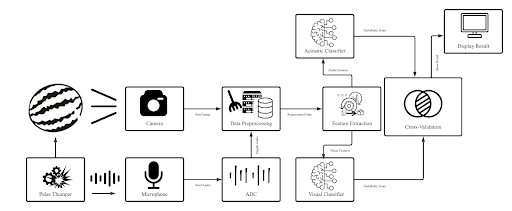
\includegraphics[width=\linewidth]{figures/system_architecture}
	\caption{System Architecture}
	\label{fig:system_arc\clearpage
    hitecture}
\end{figure}


\subsubsection{Circuit Diagram}
 
\begin{figure}[ht]
	\centering
	\includegraphics[width=\linewidth]{figures/circuit_diagram}
	\caption{Circuit Diagram}
	\label{fig:circuit_diagram}
\end{figure}
 
\subsubsection{Hardware Design}
 
This subsection describes the physical structure of the proposed system used for
watermelon ripeness analysis. The design includes a three-dimensional (3D) model to
visualize the overall structure and a two-dimensional (2D) model that presents the
dimensional layout and component placement.
\clearpage

\noindent\textbf{3D Model}
 
\vspace{6pt}
 
This section shows the arrangement of major components such as the camera
module, microphone sensor, tapping mechanism, and LCD display. The model provides a
clear visualization of how the components are integrated within the enclosure.
 
\begin{figure}[!hb]
	\centering
	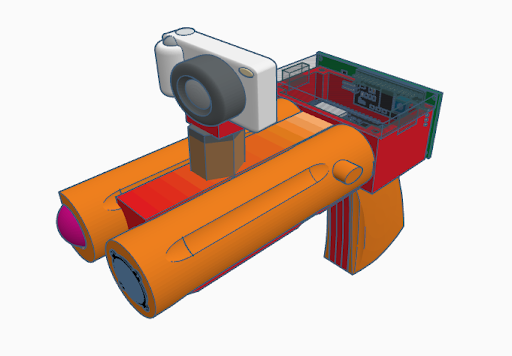
\includegraphics[width=0.65\linewidth]{figures/3d-model}
	\caption{3D Model of the proposed watermelon analysis device.}
	\label{fig:3d_model}
\end{figure}
\clearpage
 
The design ensures proper positioning of the imaging and acoustic sensing
components to enable consistent data acquisition during the ripeness detection process.

 
\noindent\textbf{2D Model}
 
\vspace{6pt}
 
The two-dimensional (2D) model of the proposed device. This section includes
multiple orthographic views, such as the top, side, front, and back views, to illustrate
the structural layout of the hardware system. These views provide a clearer
representation of the device's dimensions, component placement, and overall
configuration.
 
\begin{figure}[ht]
	\centering
	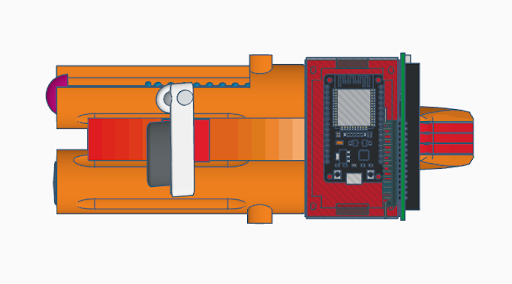
\includegraphics[width=0.75\linewidth]{figures/top_view}
	\caption{Top View}
	\label{fig:top_view}
\end{figure}
 
\begin{figure}[ht]
	\centering
	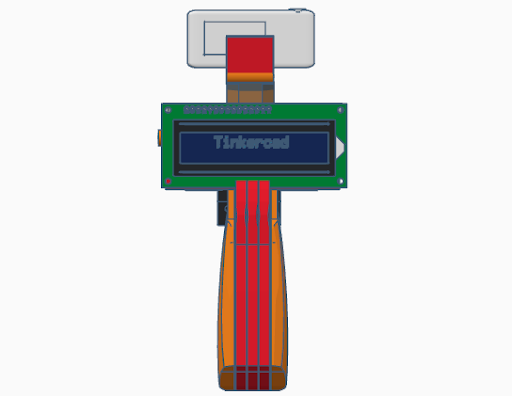
\includegraphics[width=0.75\linewidth]{figures/rear_view}
	\caption{Rear View}
	\label{fig:rear_view}
\end{figure}
 
\begin{figure}[ht]
	\centering
	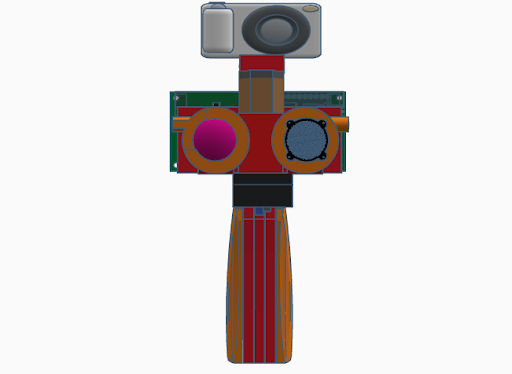
\includegraphics[width=0.75\linewidth]{figures/front_view}
	\caption{Front View}
	\label{fig:front_view}
\end{figure}
 
\begin{figure}[ht]
	\centering
	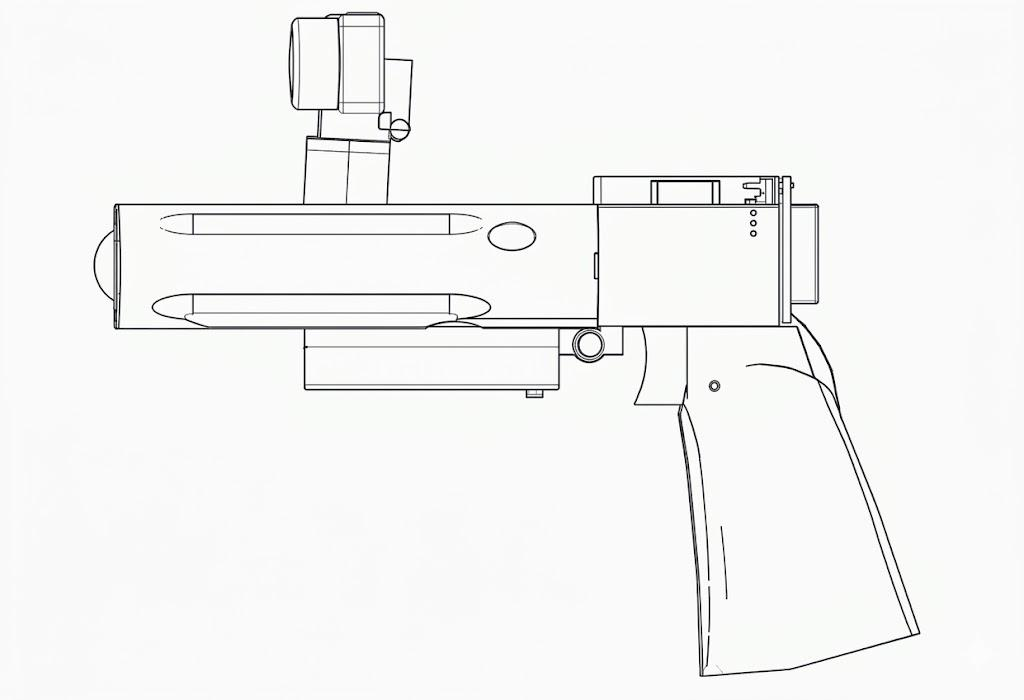
\includegraphics[width=0.75\linewidth]{figures/side_view}
	\caption{Side View}
	\label{fig:side_view}
\end{figure}
 
\newpage
 
\vspace{6pt}
 
\begin{figure}[ht]
	\centering
	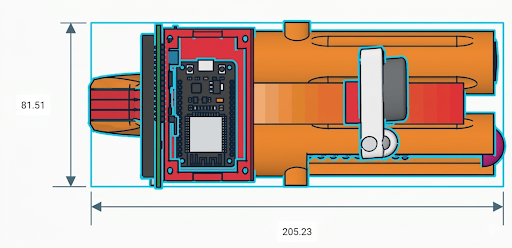
\includegraphics[width=0.75\linewidth]{figures/m&d1}
	\caption{}
	\label{fig:measurements_top}
\end{figure}
 
\begin{figure}[ht]
	\centering
	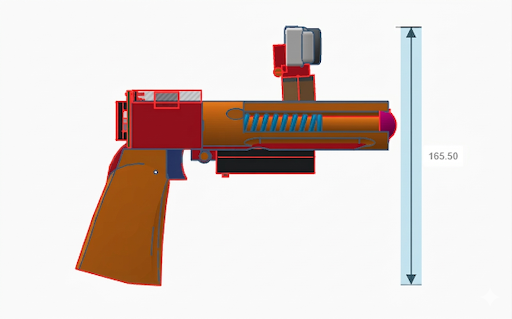
\includegraphics[width=0.75\linewidth]{figures/m&d2}
	\caption{Measurements and Dimensions}
	\label{fig:measurements_side}

\end{figure}
\clearpage
 
\subsection{Software Development}
 
\subsubsection{Software Architecture}
 
\paragraph*{Context Level Diagram}
 
\begin{figure}[ht]
	\centering
	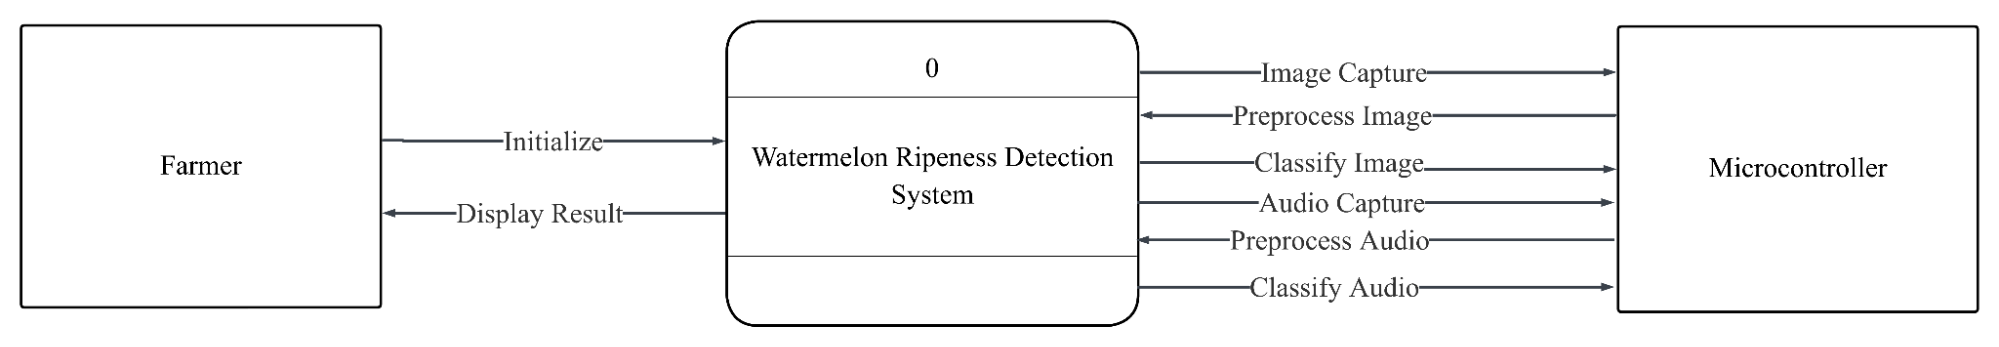
\includegraphics[width=\linewidth]{figures/context_level_diagram}
	\caption{Context Level Diagram}
	\label{fig:context_level_diagram}
\end{figure}
 
\section{Another Section}
 
\myequation{Some text}
 
\section{Tables}
 
\begin{center}
	\begin{longtable}{|l|l|l|}
		\caption{A sample long table.} \label{tab:long} \\
		
		\hline \multicolumn{1}{|c|}{\textbf{First column}} & \multicolumn{1}{c|}{\textbf{Second column}} & \multicolumn{1}{c|}{\textbf{Third column}} \\ \hline 
		\endfirsthead
		
		\multicolumn{3}{c}%
		{{\bfseries \tablename\ \thetable{} -- continued from previous page}} \\
		\hline \multicolumn{1}{|c|}{\textbf{First column}} & \multicolumn{1}{c|}{\textbf{Second column}} & \multicolumn{1}{c|}{\textbf{Third column}} \\ \hline 
		\endhead
		
		\hline \multicolumn{3}{|r|}{{Continued on next page}} \\ \hline
		\endfoot
		
		\hline \hline
		\endlastfoot
		
		One & abcdef ghjijklmn & 123.456778 \\
		One & abcdef ghjijklmn & 123.456778 \\
		One & abcdef ghjijklmn & 123.456778 \\
		One & abcdef ghjijklmn & 123.456778 \\
		One & abcdef ghjijklmn & 123.456778 \\
		One & abcdef ghjijklmn & 123.456778 \\
		One & abcdef ghjijklmn & 123.456778 \\
		One & abcdef ghjijklmn & 123.456778 \\
		One & abcdef ghjijklmn & 123.456778 \\
		One & abcdef ghjijklmn & 123.456778 \\
		One & abcdef ghjijklmn & 123.456778 \\
		One & abcdef ghjijklmn & 123.456778 \\
		One & abcdef ghjijklmn & 123.456778 \\
		One & abcdef ghjijklmn & 123.456778 \\
		One & abcdef ghjijklmn & 123.456778 \\
		One & abcdef ghjijklmn & 123.456778 \\
		One & abcdef ghjijklmn & 123.456778 \\
		One & abcdef ghjijklmn & 123.456778 \\
		One & abcdef ghjijklmn & 123.456778 \\
		One & abcdef ghjijklmn & 123.456778 \\
		One & abcdef ghjijklmn & 123.456778 \\
		One & abcdef ghjijklmn & 123.456778 \\
		One & abcdef ghjijklmn & 123.456778 \\
		One & abcdef ghjijklmn & 123.456778 \\
		One & abcdef ghjijklmn & 123.456778 \\
		One & abcdef ghjijklmn & 123.456778 \\
		One & abcdef ghjijklmn & 123.456778 \\
		One & abcdef ghjijklmn & 123.456778 \\
		One & abcdef ghjijklmn & 123.456778 \\
		One & abcdef ghjijklmn & 123.456778 \\
		One & abcdef ghjijklmn & 123.456778 \\
		One & abcdef ghjijklmn & 123.456778 \\
		One & abcdef ghjijklmn & 123.456778 \\
		One & abcdef ghjijklmn & 123.456778 \\
		One & abcdef ghjijklmn & 123.456778 \\
		One & abcdef ghjijklmn & 123.456778 \\
		One & abcdef ghjijklmn & 123.456778 \\
		One & abcdef ghjijklmn & 123.456778 \\
		One & abcdef ghjijklmn & 123.456778 \\
		One & abcdef ghjijklmn & 123.456778 \\
		One & abcdef ghjijklmn & 123.456778 \\
		One & abcdef ghjijklmn & 123.456778 \\
		One & abcdef ghjijklmn & 123.456778 \\
		One & abcdef ghjijklmn & 123.456778 \\
		One & abcdef ghjijklmn & 123.456778 \\
		One & abcdef ghjijklmn & 123.456778 \\
		One & abcdef ghjijklmn & 123.456778 \\
		One & abcdef ghjijklmn & 123.456778 \\
		One & abcdef ghjijklmn & 123.456778 \\
		One & abcdef ghjijklmn & 123.456778 \\
		One & abcdef ghjijklmn & 123.456778 \\
		One & abcdef ghjijklmn & 123.456778 \\
		One & abcdef ghjijklmn & 123.456778 \\
		One & abcdef ghjijklmn & 123.456778 \\
		One & abcdef ghjijklmn & 123.456778 \\
		One & abcdef ghjijklmn & 123.456778 \\
		One & abcdef ghjijklmn & 123.456778 \\
		One & abcdef ghjijklmn & 123.456778 \\
		One & abcdef ghjijklmn & 123.456778 \\
		One & abcdef ghjijklmn & 123.456778 \\
		One & abcdef ghjijklmn & 123.456778 \\
		One & abcdef ghjijklmn & 123.456778 \\
		One & abcdef ghjijklmn & 123.456778 \\
		One & abcdef ghjijklmn & 123.456778 \\
		One & abcdef ghjijklmn & 123.456778 \\
		One & abcdef ghjijklmn & 123.456778 \\
		One & abcdef ghjijklmn & 123.456778 \\
		One & abcdef ghjijklmn & 123.456778 \\
		One & abcdef ghjijklmn & 123.456778 \\
		One & abcdef ghjijklmn & 123.456778 \\
		One & abcdef ghjijklmn & 123.456778 \\
		One & abcdef ghjijklmn & 123.456778 \\
		One & abcdef ghjijklmn & 123.456778 \\
		One & abcdef ghjijklmn & 123.456778 \\
		One & abcdef ghjijklmn & 123.456778 \\
		One & abcdef ghjijklmn & 123.456778 \\
		One & abcdef ghjijklmn & 123.456778 \\
		One & abcdef ghjijklmn & 123.456778 \\
		One & abcdef ghjijklmn & 123.456778 \\
		One & abcdef ghjijklmn & 123.456778 \\
	\end{longtable}
\end{center}
\begin{table}[ht]
	\centering
	\caption{Sample Data Table}
	\label{tab:sample}
	\begin{tabular}{l c r}
		\toprule
		\textbf{Item} & \textbf{Quantity} & \textbf{Price (\$)} \\
		\midrule
		Apples & 10 & 0.50 \\
		Bananas & 5 & 0.30 \\
		Cherries & 20 & 1.20 \\
		Dates & 50 & 2.50 \\
		\bottomrule
	\end{tabular}
\end{table}
\section{Images}
\begin{figure}
	\centering
	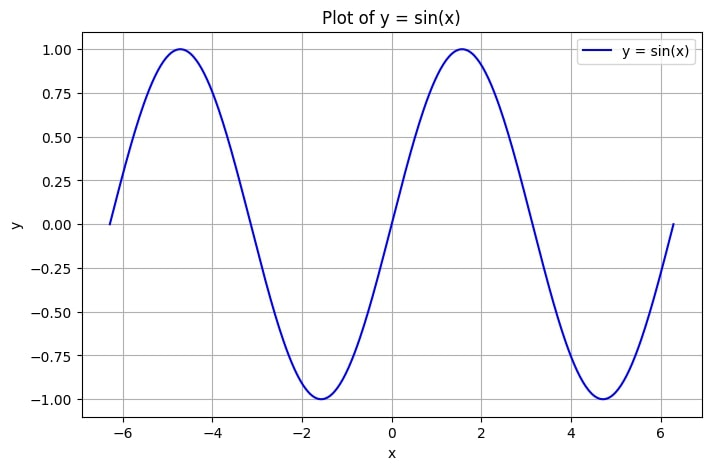
\includegraphics[width=0.7\linewidth]{figures/sinegraph}
	\caption{}
	\label{fig:sinegraph}
\end{figure}
 
\begin{figure}[h]
	\centering
	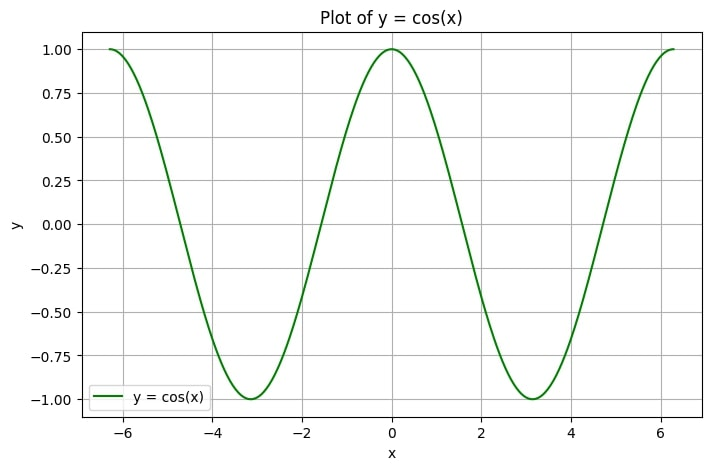
\includegraphics[height=0.3\textheight]{figures/cosinegraph}
	\caption[Cosine Graph]{Cosine Graph}
	\label{fig:cosinegraph}
\end{figure}
}

